\section{Open Question}\label{openq}
    Dopo un'analisi preliminare sui contenuti del dibattito e una caratterizzazione delle due parti contrapposte, definite in base alla misura continua dell'opinione, $C_{u}$, illustriamo qui le diverse analisi condotte sulla nostra rete al fine di investigare e quantificare la presenza di \textit{echo chambers}, il loro processo di formazione, con particolare attenzione all'influenza dei nodi "importanti" della rete. 
    
    \subsection{Contenuto e contesto del dibattito}
    
    \begin{figure}[b]
        \centering
        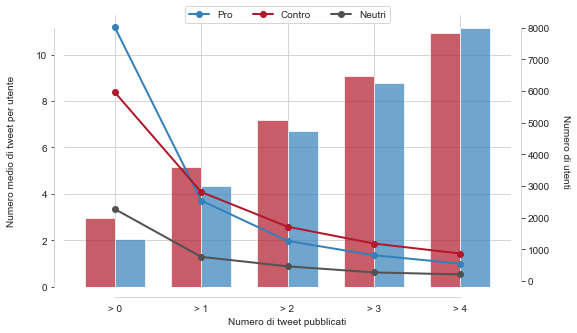
\includegraphics[scale=.36]{7_Open_question/ntweets.png}
        \caption{Il grafico a linee (scala a destra) mostra il numero di utenti a favore, contrari e neutri, che hanno pubblicato almeno 1 tweet (> 0), almeno 2 tweet (> 1) e così via. Il grafico a barre (scala a sinistra) mostra il numero medio di tweet pubblicati per utente contrario (in rosso) e a favore (in blu).}
        \label{andamentotweet}
    \end{figure}
    
    Dei 16675 nodi della  rete, il 97\% (16235) corrisponde effettivamente ad autori di tweet e non ad account esclusivamente menzionati. Di questi, 8009 sono stati classificati come a favore dell'inginocchiarsi ($C_{u} \leq -0.5$) e 5957 come contrari ($C_{u} \geq 0.5$). 
    Considerando gli autori di almeno due tweet, gli utenti contrari superano in numero quelli a favore (fig. \ref{andamentotweet}). Inoltre, il tasso di pubblicazione per le due parti appare tendenzialmente diverso, con 16510 tweets pubblicati dai sostenitori, in media circa 2 tweets per utente, e 17668 postati dal gruppo dei contrari, circa 3 tweets per utente.   
    
    Un'ulteriore differenza comportamentale tra le due parti è ben rappresentata in figura \ref{almenotot}, in cui mostriamo la distribuzione delle opinioni $C_{u}$ degli utenti. Innanzitutto, si evidenzia chiaramente la netta divisione in due gruppi con orientamenti opposti, con un ridotto numero di utenti aventi una posizione neutra o non classificabile. I boxplot, inoltre, mettono in luce l'asimmetria %rispetto a $C_{u}=0$ 
    di tale distribuzione, già suggerita dall'analisi visiva dell'istogramma: per $C_{u}>0.5$ gli utenti hanno opinioni mediamente più estreme, mentre per $C_{u}<-0.5$ si hanno valori più moderati. 
    
    \begin{center}
        \animategraphics[controls,scale=0.45]{2}{7_Open_question/distribuzione opinioni almeno}{5}{1}
        \vspace{2mm}
        \begin{figure}[h!]
        \caption{In basso: numero di utenti* in funzione del valore di classificazione. In alto: boxplots della distribuzione delle opinioni non neutre, da 0.5 al limite massimo ($\pm 3$). }
        \label{almenotot}
        \end{figure}
    \end{center}
    \vspace{-5mm}
    
    \begin{figure*}[b]
        \centering
        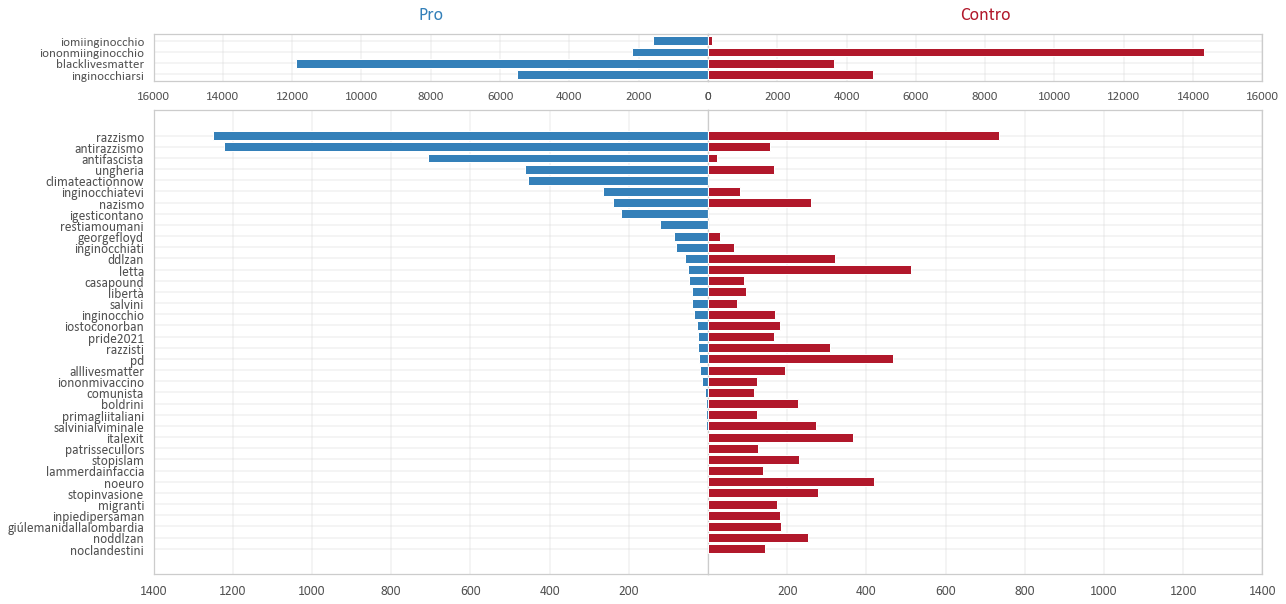
\includegraphics[scale=.34]{7_Open_question/distr hashtag senza neutri.png}
        \caption{Frequenza degli hashtag, unificati nella stessa forma normalizzata, ordinati per utilizzo da parte dei sostenitori.}
        \label{distr_hash}
    \end{figure*}
    
    Tale risultato conferma quanto già suggerito dalle operazioni di classificazione effettuate sugli hashtag (par. \ref{subsection:class}), in cui appariva evidente un maggiore utilizzo di hashtag dichiaratamente contrari al gesto ($C_{h}=3$), a differenza degli hashtag utilizzati dai sostenitori, i quali - più che a sostegno del gesto in sé - pongono l'accento sui motivi etici e morali dietro di esso. Infatti, se gli utenti contrari al gesto hanno utilizzato l'hashtag \texttt{\#iononmiinginocchio} più di 14000 volte, la controparte ha twittato utilizzando l'hashtag \texttt{\#iomiinginocchio} meno di 2000 volte, preferendo invece l'hashtag \texttt{\#blacklivesmatter} (fig. \ref{distr_hash}). Inoltre, in certa misura, sia i sostenitori che i contrari al gesto hanno utilizzato l'hashtag "bandiera" della controparte per parlarne e, spesso, prenderne le distanze.
    
    La sezione in basso di figura \ref{distr_hash} mostra la differenza nell'utilizzo degli hashtag più popolari da parte delle due fazioni, al netto degli hashtag neutri o non pertinenti, che sono stati opportunamente esclusi da questo studio, ordinati rispetto all'utilizzo da parte dei sostenitori. È interessante notare che \texttt{\#razzismo} sia stato utilizzato in modo consistente da entrambe le parti, indice del risvolto etico della questione discussa. Al contempo, numerosi sono i richiami a questioni politiche e sociali, principalmente tra gli utenti contrari al gesto: infatti, se tra gli hashtag maggiormente utilizzati dai sostenitori del gesto troviamo per lo più slogan contro il razzismo e contro le dittature, gli hashtag maggiormente utilizzati dai contrari al gesto spaziano su diverse questioni di attualità, dall'immigrazione (\texttt{\#stopinvasione}) al DDL Zan (\texttt{\#noddlzan} e all'anti-europeismo (\texttt{\#italexit}), toccando persino le vaccinazioni anti Covid-19 (\texttt{\#iononmivaccino}).   
    
    \subsection{Siamo di fronte a delle echo chambers?} \label{subsection:echochamb}
    
    \begin{figure*}[pb]
        \centering
        \begin{subfigure}{.4\textwidth}
            \centering
            \caption{}
            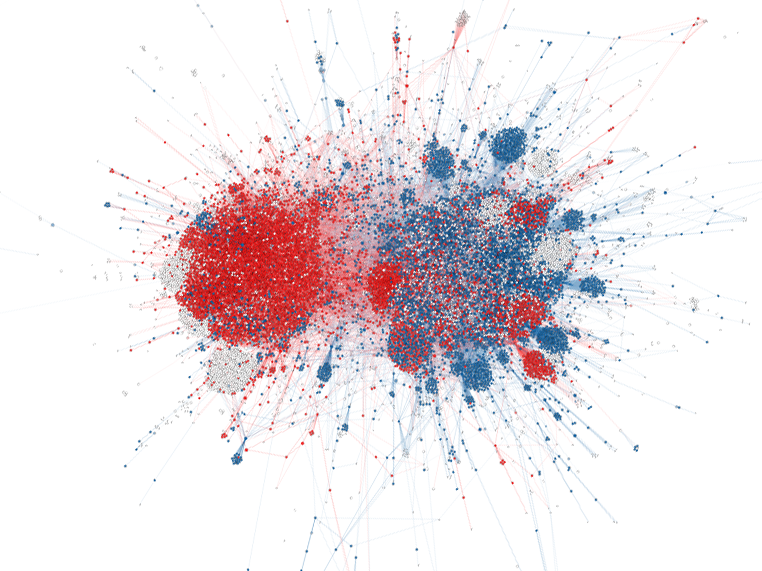
\includegraphics[width=7cm]{7_Open_question/rete_vecchia_cut.png}
            \label{echo_chamber_not_clean}
        \end{subfigure}
        \centering
        \begin{subfigure}{.4\textwidth}
            \centering
            \caption{}
            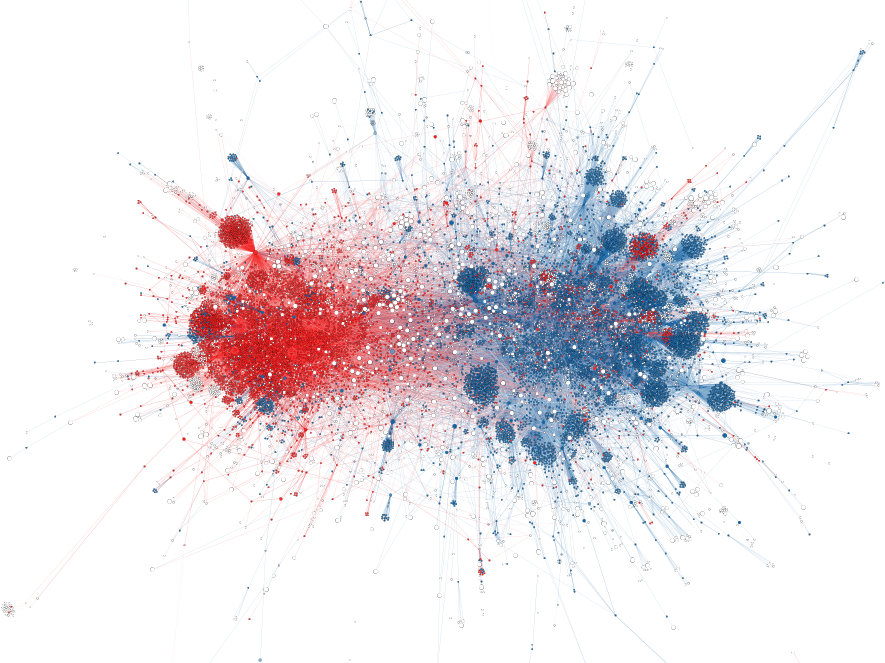
\includegraphics[width=7cm]{7_Open_question/rete_nuova_cut.png}
            \label{echo_chamber_clean}
        \end{subfigure}
        \vspace{-5mm}
        \caption{Visualizzazione della rete effettuata con l'algoritmo di layout ForceAtlas2 fornito da Geohi, prima (\subref{echo_chamber_not_clean}) e dopo (\subref{echo_chamber_clean}) la correzione degli errori di classificazione più influenti. In \subref{echo_chamber_clean}, la dimensione dei nodi aumenta in base all'attributo \texttt{vip}, ovvero al numero di followers.}
        \label{echochambers}
    \end{figure*}
    
    Per rispondere a questa domanda, abbiamo utilizzato la rappresentazione proposta da ForceAtlas2, un algoritmo di layout grafico per la visualizzazione delle reti sviluppato per il software Gephi, in cui zone più connesse risultano spazialmente più vicine e viceversa (fig. \ref{echo_chamber_not_clean}). 
    I colori utilizzati rappresentano l'opinione in merito al gesto come definita in \ref{subsection:class}: blu per i sostenitori, rosso per i contrari, bianco per i neutri o non classificabili. 
    
    Dall’immagine risulta evidente una separazione spaziale della rete in due agglomerati, corrispondente in buona misura alla classificazione cromatica. Permangono, tuttavia, diverse aree rosse nell’agglomerato blu e grosse aree bianche in entrambe le parti. L'analisi di queste zone ha evidenziato degli errori nella classificazione di alcuni tweets divenuti virali, che quindi hanno influito sulla classificazione di ogni utente che li ha ritweettati.
    Tra questi, esemplare è il caso del tweet a sostegno del gesto\footnote{ 26 giugno 2021, Roberto Saviano (@robertosaviano), "Si inginocchia chi vuole rendere rispetto a chi è vittima, segnare simbolicamente il proprio impegno perché le cose cambino. Quand'è che esattamente ha iniziato a farci schifo il buon esempio?     \#Inginocchiarsi \#IoNonMiInginocchio"} pubblicato dall'utente @robertosaviano, in cui l'hashtag \texttt{\#iononmiinginocchio} ($C_{h} = +3$), utilizzato per fare riferimento al dibattito, ha generato una classificazione errata. Tramite un'ispezione visiva del grafo su Gephi, abbiamo individuato gli errori di classificazione con maggiore impatto sulla rete e modificato manualmente la classificazione dei tweet responsabili dell'errore, che elenchiamo di seguito:
    
    \begin{itemize}
        \item $C_{t}=-3$ per i tweet di @robertosaviano, @ProfCampagna, @pietroraffa, @LuciaCaprig e @manginobrioches in cui si sono espressamente schierati a favore del gesto; 
        \item $C_{t}=-1$ per i tweet di @PBerizzi e @MarcoNoel19 in cui hanno espresso posizioni vicine ai motivi dietro al gesto;
        \item  $C_{t}=1$ per i tweet di @lefrasidiosho e @LeonardoPanetta in cui hanno espresso un'opinione lontana dai motivi del gesto o tendenzialmente contraria.
    \end{itemize}
    
    Queste operazioni hanno condotto ad un sensibile miglioramento nella caratterizzazione delle due echo chambers (fig. \ref{echo_chamber_clean}). 
    
    \begin{center}
        \animategraphics[controls, scale=0.45]{2}{7_Open_question/Density_2tweets_}{0}{6}
        \vspace{1mm}
        \begin{figure}[h!]
        \caption{\textit{Contour map} per opinione media dei vicini $C_{N(u)}$ rispetto all'opinione media di un utente $C_{u}$. I colori rappresentano la densità di utenti: più chiaro è, maggiore è il numero di utenti. Per la distribuzione di probabilità di $C_{U}$ fare riferimento al penultimo grafico in figura \ref{almenotot} in quanto vengono considerati solo gli utenti autori di almeno 2 post (3370).}
        \label{Contourmaps}
        \end{figure}
    \end{center}
    \vspace{-5mm}
    
    
    
    Uno dei modi per quantificare la presenza di camere d'eco è mettere in relazione l'opinione di un utente con l'inclinazione dei suoi vicini. A livello topologico, ci aspettiamo che un nodo \textit{u} con una data opinione $C_{u}$ sia connesso con nodi con opinioni prossime a $C_{u}$. Abbiamo così definito, per ogni utente \textit{u}, l'opinione media dei suoi vicini, $C_{N(u)}$. L'ultima immagine della figura \ref{Contourmaps} mostra una forte correlazione tra l'opinione di un utente \textit{u} e la posizione dei suoi vicini più prossimi $C_{N(u)}$. Il coefficiente di correlazione di Pearson r è 0.84, dunque statisticamente significativo, con $\text{\textit{p-value}} \simeq 0$. Questa proprietà topologica della rete conferma la presenza di camere d'eco: gli utenti che esprimono tendenze sia a favore che contrarie al gesto hanno maggiori probabilità di interagire con utenti che condividono la loro opinione.
    
    Un secondo indice della tendenza dei nodi della nostra rete a creare legami con nodi con caratteristiche simili è l'\textit{assortative mixing} - o omofilia, in reti generiche - calcolata utilizzando il coefficiente di \textit{assortativity}:
    \begin{equation}
        r=\frac{\sum_i e_{ii}-\sum_i a_i b_i}{1-\sum_i a_i b_i}
        \label{omofily_coefficient}
    \end{equation}
    L'intervallo di opinioni è stato discretizzato in tre differenti fazioni: a favore, con $C_{u}\leq-0.5$, contrari, con $C_{u}\geq0.5$, e neutri, con opinioni comprese tra -0.5 e 0.5. Tale coefficiente è pari a 0.22, valore maggiore di 0, che conferma la tendenza a formare connessioni tra nodi con caratteristiche simili.
    
    \begin{figure}
        \centering
        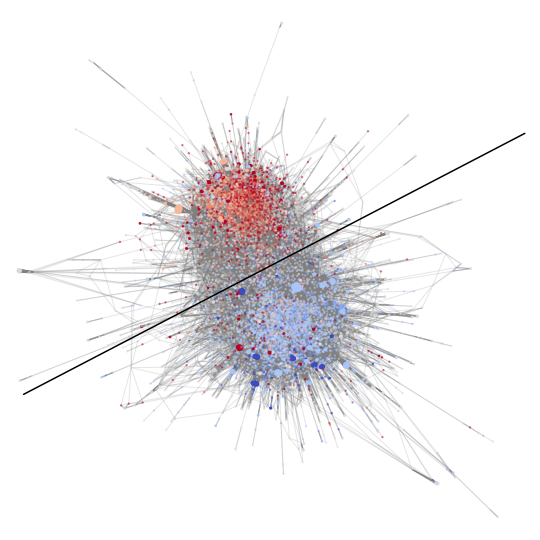
\includegraphics[width=6cm] {7_Open_question/echo_chamber_division.png}
        \caption{Separazione dei due agglomerati correlati, relativamente, con la maggior presenza di nodi della fazione rossa e blu.}
        \label{echo_chamber_division}
    \end{figure}
    
    Per analizzare la struttura e la composizione interna alle due camere d'eco, abbiamo diviso la rete separandole l'una dall'altra. Nello specifico, tramite la libreria fa2 \_v0.3.5, implementazione Python del layout grafico Force Atlas 2 progettato per Gephi, è stata generata una spazializzazione 2D del nostro grafo (fig. \ref{echo_chamber_division}), su cui è stata individuata e tracciata la retta che meglio divideva le due camere d'eco; infine, sono stati generati due sottografi, uno con i nodi e i link della sezione al di sopra della retta (sottografo R), e uno con quelli al di sotto di essa (sottografo B). Al netto delle componenti sconnesse, il sottografo B risulta essere più grande (9262 nodi, 27573 link \textit{vs} 6746 nodi, 21163 link), ma meno denso (0.0006 \textit{vs} 0.0009) del sottografo R, che registra valori maggiori anche per quanto riguarda il grado medio (5.95 \textit{vs} 6.27) e il valore di transitività (0.012 \textit{vs} 0.019). Inoltre, se in entrambi i sottografi si registra una percentuale di nodi con opinione neutra molto simile ($\simeq 22\%$), il sottografo R, mediamente contrario al gesto ($\bar{C}_{u} = 1.24$), ospita una percentuale più alta di nodi della fazione opposta: 11.4\% di utenti a favore in R contro l'8.7\% di utenti contrari nel sottografo B, in cui il valore medio dell'opinione $\bar{C}_{u}$ è di circa -0.81. Infine, è stato stimato a 3196 il numero di link che intercorrono tra le due \textit{echo chambers}, poco più del 6\% di tutti i link del grafo originario.
    
    \subsection{Chi ha preso parte al dibattito?}\label{who}
    Un'ulteriore analisi effettuata sui due sottografi ha riguardato lo studio degli hubs, con particolare attenzione a quelli con un alto numero di followers ($\texttt{vip} > 0$). Innanzitutto, occorre precisare che, sebbene nella rete siano presenti più di 1000 utenti con almeno 20000 followers, più dei tre quarti di essi lo sono in quanto menzionati da altri utenti.
    Diversi, ad esempio, sono stati i personaggi pubblici chiamati in causa nel dibattito, principalmente politici nella parte contraria al gesto e personaggi dello sport in quella a sostegno: da @chiellini, \textit{username} di Giorgio Chiellini, giocatore della Nazionale, criticato per la gaffe sul nazismo \cite{chiellini_nazismo}, a @marchisiocla8, Claudio Marchisio, ex-giocatore della Nazionale, oggi giornalista sportivo, che in varie occasioni ha espresso la sua vicinanza al movimento BLM \cite{marchisio}. Interessante è il caso di @EnricoLetta, segretario del Partito Democratico: intervenuto pubblicamente sulla questione chiedendo alla squadra di inginocchiarsi all'unanimità \cite{letta}, ha attirato su di sé uno sciame di critiche da parte dei contrari al gesto, venendo così "assorbito" nella camera d'eco principalmente popolata da questi ultimi, accanto ai nomi di @matteosalvinimi (Matteo Salvini, leader della Lega) e @GiorgiaMeloni (Giorgia Meloni, leader di Fratelli D'Italia).
    
    Considerando 33 \textit{hubs}, corrispondenti al primo \SI{2}{\permille} dei nodi riordinati per grado, 20 risultano essere utenti "attivi", ovvero autori di almeno un post, e molto seguiti: il 75\% di essi infatti ha più di 10000 followers e comunque nessuno scende sotto i 2000; questi utenti risultano essere principalmente account di giornalisti e scrittori. Sembrerebbe dunque che il numero di followers di un utente ricopra un ruolo molto importante nell'impatto di questi sulla rete.
    Al contempo, sebbene nella nostra rete siano presenti ben 378 utenti con un numero di followers maggiore di 200000 mila, solo 13 sono da considerarsi attivi, e addirittura solo 2 di questi ricoprono il ruolo di \textit{hub}: nel sottografo R troviamo @lefrasidiosho, account Twitter della pagina satirica Facebook "Le più belle frasi di Osho", al 7° posto nella lista ordinata degli hubs, mentre nel sottografo B, @robertosaviano, account Twitter del noto scrittore Roberto Saviano, 12° posto. Ne possiamo dedurre che, per quanto siano stati coinvolti diversi personaggi pubblici, direttamente o indirettamente, non è grazie a questi che il dibattito si è sviluppato, bensì intorno a utenti mediamente conosciuti, ma con un alto valore di \textit{user engagment}, ovvero molto attivi rispetto a questo genere di tematiche.
    
    \subsection{Quando nasce l'echo chamber?}\label{when}
    Al fine di individuare il momento della formazione delle \textit{echo chambers} e la loro evoluzione nel tempo, abbiamo adottato nuovamente la suddivisione in sette intervalli temporali adottata in \ref{dcd}.
    Come primo approccio, abbiamo riproposto lo studio della correlazione tra l’opinione di un utente $C_{u}$ e la posizione dei suoi vicini più prossimi $C_{N (u)}$, calcolata in ogni intervallo di tempo (fig. \ref{Contourmaps}). 
    
    \begin{figure}[!b]
        \centering
        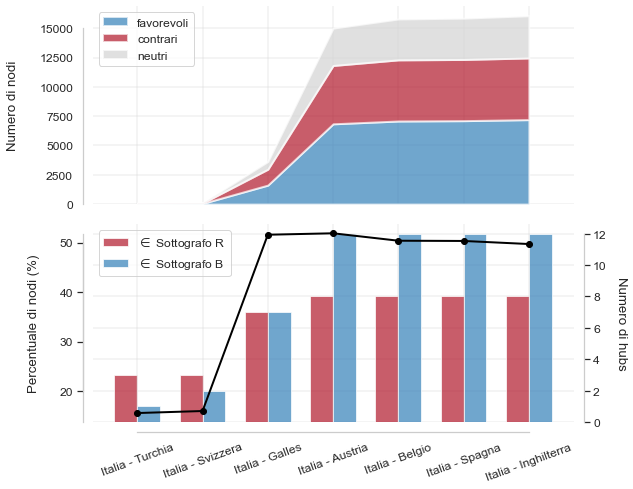
\includegraphics[scale=.34] {7_Open_question/evolutions.png}
        \caption{In alto: Lo \textit{stacked area chart} mostra la crescita della rete nel tempo in relazione all'opinione dei nodi che ne entrano a far parte. In basso: il grafico a linee (scala a sinistra) mostra la percentuale di nodi della rete collegati agli hubs. Il grafico a barre (scala a destra) mostra il numero di hubs presenti nei diversi intervalli di tempo nelle camere d'eco R (in rosso) e B (in blu).}
        \label{hubs_evolution}
    \end{figure}
    
    Risulta immediatamente evidente che, se inizialmente gli utenti si estendono in un'area molto ampia (coefficiente di Pearson $r \simeq 0.5$), con il passare del tempo, la tendenza della densità a disporsi diagonalmente si accentua gradualmente, fino a crescere in modo importante ($r=0.7$) in corrispondenza del terzo intervallo di tempo, ovvero tra Italia-Galles e Italia-Austria, e divenire statisticamente significativa ($r = 0.82$) nel quarto intervallo, tra Italia-Austria e Belgio-Italia, dopo il quale la situazione rimane pressocché inviata.

    La formazione delle camere d'eco, dunque, prende piede nei giorni che seguono Italia-Galles (terzo intervallo) per poi definirsi e stabilizzarsi in coincidenza del grande incremento del numero di nodi nella rete che si verifica nell'intervallo di tempo che intercorre tra Italia-Austria e Belgio-Italia (fig. \ref{hubs_evolution}, in alto).
    
    Si noti, inoltre, come tale intervallo abbia coinciso con la comparsa nella rete di tutti i nodi identificati come hubs "attivi", con i quali circa il 50\% dei nodi dell'intera rete ha creato collegamenti diretti (fig. \ref{hubs_evolution}, in basso). Possiamo dunque supporre che la loro presenza abbia in qualche misura contribuito da un lato alla crescita della rete, trattandosi di nodi con una capacità di \textit{user engagment} tutt'altro irrilevante, e dall'altro alla polarizzazione dell'opinione.